%!TEX root = ../TAMUTemplate.tex
%%%%%%%%%%%%%%%%%%%%%%%%%%%%%%%%%%%%%%%%%%%%%%%%%%%
%
%  New template code for TAMU Theses and Dissertations starting Fall 2016.
%
%  Author: Sean Zachary Roberson
%	 Version 3.16.09
%  Last updated 9/12/2016
%
%%%%%%%%%%%%%%%%%%%%%%%%%%%%%%%%%%%%%%%%%%%%%%%%%%%
%%%%%%%%%%%%%%%%%%%%%%%%%%%%%%%%%%%%%%%%%%%%%%%%%%%%%%%%%%%%%%%%%%%%%%
%%                           SECTION IV
%%%%%%%%%%%%%%%%%%%%%%%%%%%%%%%%%%%%%%%%%%%%%%%%%%%%%%%%%%%%%%%%%%%%%



\chapter{\uppercase {Event Reconstruction}}
\label{ch:event_reconstruction}

The CMS detector is designed to identify the various particle species which travel through it after a proton-proton collision.
As discussed in chapter~\ref{ch:LHC_CMS}, the sub-detector technologies were chosen so that particles could be identified by where they deposite their energy as well as how their trajectories change in a magnetic field.
Fig~\ref{fig:particle_flow} shows how various types of particles interact with the CMS detector.
All of the charged particles (\ie electrons, muons, and charged hadrons) will deposit some energy in the tracker, while neutral particles (\ie photons and neutral hadrons) will not.
Electrons and photons will deposit all of their energy inside of the ECAL while hadrons, both charged and neutral, will deposit most of their energy in the HCAL.
Muons are the only visible particle which will be able to travel to the muon chambers.
Neutrinos will pass through all layers of the detector unseen and their presence must be infered by missing transverse energy (\MET or \ETslash); the idea being that if the sum of the transverse momentum is not conserved, then that missing momentum must correspond to at least one unseen particle.

\begin{figure}[!hbt]
	\centering
	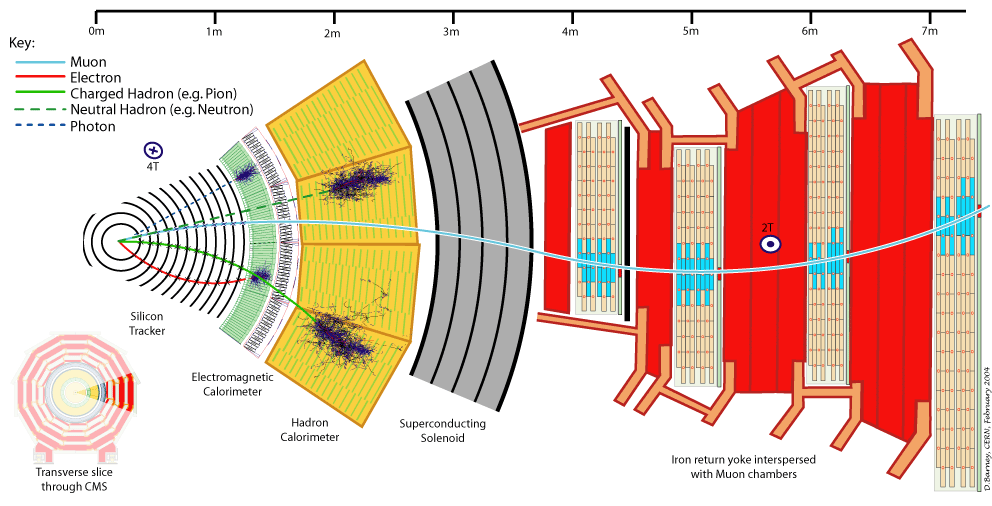
\includegraphics[width=0.95\textwidth]{\figpath/Chapter3/ParticleFlow}
	\caption{Cross-sectional view of the CMS detector with all of the sub-detectors labeled.The colored lines correspond to different particle species, which interact with different pieces of the detector and may or may not be bent by the magnetic field.}
	\label{fig:particle_flow}
\end{figure}

The process of translating abstract detector objects to physical particles takes several steps within the CMS software framework (CMSSW).
The first of this process is local reconstruction, where the various subsystems of each sub-detector create what are called reconstucted hits, or RecHits for short.
RecHits in the tracker contain information about the position of energy clusters (groups of contiguous strips or pixels which contain a signal) as well as energy deposition information which aids in particle identification.
The muon RecHits ostensibly contain information about the position of the signal.
However, the RecHits from the DTs and CSCs can be combined to form three-dimensional track segments, which also provide directional information.
The ECAL and HCAL RecHits contain information about the energy deposited, the position of those deposits, and the time at which they occured.

The next step is to process this information in a global manner, where the subsystems within each sub-detector are combined.
Pattern recongnition algorithms are run on the tracker RecHits to reconstruct the path that the particles take through the sub-detector (a.k.a tracks).
The ECAL and HCAL RecHits within a tower are summed to form ``CaloTowers'' which have a projective $\eta-\phi$ geometry.
The muon system creates ``standalone'' muons by associating RecHits and track segments with compatible radial trajectories.
This process takes into account the bending a muon undergoes before reaching and within the muon system due to the magnetic field.

At this point, all of the reconstuction information is combined to form particles that can be used for physics analysis.
The process of reconstucting and classifying every stable particle is called Particle Flow (PF) and will be discussed further in chapter~\ref{sec:particle_flow}.
This analysis focuses on electrons, muons, jets, b-jets, and \ETslash, the reconstuction of which will be described in the following sections.
Additional information about the reconstruction process beyond the scope of this thesis can be found in~\cite{TDR-software}.

\section{Tracks and Vetices}
\label{sec:tracks_and_vertices}



\section{Particle Flow}
\label{sec:particle_flow}

























In longer papers, the particle-flow algorithm can be described in more detail:

The global event reconstruction (also called particle-flow event reconstruction~\cite{CMS-PAS-PFT-09-001,CMS-PAS-PFT-10-001}) consists of reconstructing and identifying each individual particle with an optimized combination of all subdetector information.
In this process, the identification of the particle type (photon, electron, muon, charged hadron, neutral hadron) plays an important role in the determination of the particle direction and energy.
Photons (\eg coming from \Pgpz\ decays or from electron bremsstrahlung) are identified as ECAL energy clusters not linked to the extrapolation of any charged particle trajectory to the ECAL.
Electrons (\eg coming from photon conversions in the tracker material or from \cPqb-hadron semileptonic decays) are identified as a primary charged particle track and potentially many ECAL energy clusters corresponding to this track extrapolation to the ECAL and to possible bremsstrahlung photons emitted along the way through the tracker material.
Muons (\eg from \cPqb-hadron semileptonic decays) are identified as a track in the central tracker consistent with either a track or several hits in the muon system, associated with an energy deficit in the calorimeters.
Charged hadrons are identified as charged particle tracks neither identified as electrons, nor as muons.
Finally, neutral hadrons are identified as HCAL energy clusters not linked to any charged hadron trajectory, or as ECAL and HCAL energy excesses with respect to the expected charged hadron energy deposit.

The energy of photons is directly obtained from the ECAL measurement, corrected for zero-suppression effects.
The energy of electrons is determined from a combination of the track momentum at the main interaction vertex, the corresponding ECAL cluster energy, and the energy sum of all bremsstrahlung photons attached to the track.
The energy of muons is obtained from the corresponding track momentum.
The energy of charged hadrons is determined from a combination of the track momentum and the corresponding ECAL and HCAL energy, corrected for zero-suppression effects and for the response function of the calorimeters to hadronic showers.
Finally, the energy of neutral hadrons is obtained from the corresponding corrected ECAL and HCAL energy.


\section{Electrons}

The electron momentum is estimated by combining the energy measurement in the ECAL with the momentum measurement in the tracker.The momentum resolution for electrons with $\pt \approx 45\GeV$ from $\Z \rightarrow \Pe \Pe$ decays ranges from 1.7\% for nonshowering electrons in the barrel region to 4.5\% for showering electrons in the endcaps~\cite{Khachatryan:2015hwa}.

The dielectron mass resolution for $\Z \rightarrow \Pe \Pe$ decays when both electrons are in the ECAL barrel is 1.9\%, and is 2.9\% when both electrons are in the endcaps. The electron momenta are estimated by combining energy measurements in the ECAL with momentum measurements in the tracker~\cite{Khachatryan:2015hwa}. 

\section{Muons}

\section{Jets}

When combining information from the entire detector, the jet energy resolution amounts typically to 15\% at 10\GeV, 8\% at 100\GeV, and 4\% at 1\TeV, to be compared to about 40\%, 12\%, and 5\% obtained when the ECAL and HCAL calorimeters alone are used.


Traditional calorimetric jets are reconstructed offline from the energy deposits in the calorimeter towers, clustered by the anti-$k_\mathrm{t}$ algorithm~\cite{Cacciari:2008gp, Cacciari:2011ma} with a size parameter of 0.4. In this process, the contribution from each calorimeter tower is assigned a momentum, the absolute value and the direction of which are given by the energy measured in the tower, and the coordinates of the tower. The raw jet energy is obtained from the sum of the tower energies, and the raw jet momentum by the vectorial sum of the tower momenta, which results in a nonzero jet mass. The raw jet energies are then corrected to establish a relative uniform response of the calorimeter in $\eta$ and a calibrated absolute response in transverse momentum \pt. 

 The particle-flow algorithm can be described in short form as:

The particle-flow event algorithm reconstructs and identifies each individual particle with an optimized combination of information from the various elements of the CMS detector. The energy of photons is directly obtained from the ECAL measurement, corrected for zero-suppression effects. The energy of electrons is determined from a combination of the electron momentum at the primary interaction vertex as determined by the tracker, the energy of the corresponding ECAL cluster, and the energy sum of all bremsstrahlung photons spatially compatible with originating from the electron track. The energy of muons is obtained from the curvature of the corresponding track. The energy of charged hadrons is determined from a combination of their momentum measured in the tracker and the matching ECAL and HCAL energy deposits, corrected for zero-suppression effects and for the response function of the calorimeters to hadronic showers. Finally, the energy of neutral hadrons is obtained from the corresponding corrected ECAL and HCAL energy.

to be followed by these other lines, after mentioning the anti-\kt algorithm:

Jet momentum is determined as the vectorial sum of all particle momenta in the jet, and is found from simulation to be within 5 to 10\% of the true momentum over the whole \pt spectrum and detector acceptance. An offset correction is applied to jet energies to take into account the contribution from additional proton-proton interactions within the same or nearby bunch crossings. Jet energy corrections are derived from simulation, and are confirmed with in situ measurements of the energy balance in dijet and photon + jet events. Additional selection criteria are applied to each event to remove spurious jet-like features originating from isolated noise patterns in certain HCAL regions.

In some papers, you would want to add some performance numbers:

The jet energy resolution amounts typically to 15\% at 10\GeV, 8\% at 100\GeV, and 4\% at 1\TeV, to be compared to about 40\%, 12\%, and 5\% obtained when the calorimeters alone are used for jet clustering.

For each event, hadronic jets are clustered from these reconstructed particles with the infrared and collinear safe anti-\kt algorithm, operated with a size parameter $R$ of 0.4. The jet momentum is determined as the vectorial sum of all particle momenta in this jet, and is found in the simulation to be within 5 to 10\% of the true momentum over the whole \pt spectrum and detector acceptance. Jet energy corrections are derived from the simulation, and are confirmed with in situ measurements with the energy balance of dijet and photon + jet events~\cite{Chatrchyan:2011ds}. The jet energy resolution amounts typically to 15\% at 10\GeV, 8\% at 100\GeV, and 4\% at 1\TeV, to be compared to about 40\%, 12\%, and 5\% obtained when the calorimeters alone are used for jet clustering. 

\section{Missing Transverse Energy}


\section{Event Generation}

\section{Detector Simulation}